\documentclass[12pt,a4paper]{article}

\usepackage{fontspec}
\usepackage{polyglossia}
\setmainlanguage{russian}
\setotherlanguage{english}
\setmainfont{Times New Roman}
\newfontfamily\cyrillicfont{Times New Roman}
\newfontfamily\cyrillicfonttt{DejaVu Sans Mono}
\usepackage{geometry}
\geometry{a4paper, top=2cm, bottom=2cm, left=3cm, right=1.5cm}
\usepackage{setspace}
\onehalfspacing
\usepackage{indentfirst}
\setlength{\parindent}{1.25cm}
\usepackage{titlesec}
\usepackage{tocloft}
\usepackage{booktabs}
\usepackage{longtable}
\usepackage{array}
\usepackage{caption}
\usepackage{float}
\usepackage{graphicx}
\usepackage{hyperref}
\usepackage{url}
\usepackage{fancyhdr}
\usepackage{enumitem}
\usepackage{amsmath}

\hypersetup{hidelinks}
\pagestyle{fancy}
\fancyhf{}
\fancyfoot[C]{\thepage}
\renewcommand{\headrulewidth}{0pt}
\titleformat{\section}{\bfseries\large}{\thesection.}{0.5em}{}
\titleformat{\subsection}{\bfseries\normalsize}{\thesubsection.}{0.5em}{}
\captionsetup{font=small, labelfont=bf}
\setlist{nosep}
\sloppy

\begin{document}

\begin{titlepage}
\thispagestyle{empty}
\begin{center}
МИНИСТЕРСТВО НАУКИ И ВЫСШЕГО ОБРАЗОВАНИЯ РОССИЙСКОЙ ФЕДЕРАЦИИ

\vspace{0.8cm}
федеральное государственное бюджетное образовательное учреждение высшего образования\\
«Новгородский государственный университет имени Ярослава Мудрого»

\vspace{3.5cm}
{\bfseries НАУЧНО-ИССЛЕДОВАТЕЛЬСКАЯ РАБОТА}

\vspace{1.2cm}
{\bfseries «Методика адаптации моделей компьютерного зрения для контроля качества литых изделий на edge-устройствах с различными ресурсными ограничениями»}
\end{center}

\vspace{3cm}
\begin{flushright}
Выполнил магистрант:\\
\mbox{Филиппов Иван Иванович}

\vspace{0.8cm}
Научный руководитель, доцент:\\
\mbox{Телина Ирина Сергеевна}
\end{flushright}

\vfill
\begin{center}
2026, Великий Новгород
\end{center}
\end{titlepage}

\tableofcontents
\newpage

\section*{Введение}
\addcontentsline{toc}{section}{Введение}

Визуальный контроль качества является одной из ключевых задач промышленной автоматизации. Для литых изделий характерны дефекты поверхности, формы или структуры, которые могут быть выявлены по изображению детали. Ошибка контроля может приводить к двум типам последствий: пропуск дефектной детали и ошибочная отправка годной детали на дополнительную проверку. В промышленной постановке первый тип ошибки обычно более критичен, поскольку дефектное изделие может попасть на следующий этап производства или к конечному потребителю.

Современные модели компьютерного зрения позволяют достигать высокого качества в задачах классификации изображений. Однако прямая переносимость таких моделей на производственные edge-устройства ограничена аппаратными ресурсами. Одни сценарии допускают использование персонального компьютера, другие требуют работы на одноплатном компьютере уровня Raspberry Pi, а наиболее жесткие сценарии предполагают микроконтроллерный режим уровня OpenMV. Эти профили различаются по доступной памяти, вычислительной мощности, допустимой задержке и поддерживаемым форматам моделей.

Проблематика исследования состоит в необходимости не просто обучить точную модель классификации дефектов, а построить воспроизводимую методику адаптации модели к разным ресурсным профилям. Такая методика должна учитывать качество классификации, размер модели, задержку инференса, формат TFLite/INT8 и возможность отправки неуверенных случаев на ручную проверку.

Объектом исследования являются модели компьютерного зрения для промышленного визуального контроля качества. Предметом исследования является методика адаптации моделей компьютерного зрения к edge-устройствам с различными ресурсными ограничениями.

Гипотеза исследования заключается в том, что легковесная модель после адаптации и exact TFLite INT8-конвертации может сохранить приемлемое качество выявления дефектов на более строгом deduplicated split при радикальном уменьшении размера модели.

Актуальность работы определяется потребностью промышленности в переносимых и экономичных системах визуального контроля. На практике важно не только получить высокую accuracy на тестовой выборке, но и понимать, насколько модель пригодна для исполнения на ограниченном устройстве, каков риск пропуска дефектов и как меняется качество после квантизации.

Научная новизна состоит в resource-aware методике адаптации: используется deduplicated-валидация, сравниваются PC/SBC/micro-edge профили, выполняется exact TFLite INT8-конвертация micro-edge модели и совместно анализируются качество, размер, latency и confidence-based triage. При этом не утверждается, что задача классификации дефектов литья решена впервые; вклад работы состоит в строгом и воспроизводимом сравнении качества и ресурсной стоимости.

Цель работы: разработать и экспериментально проверить методику адаптации моделей компьютерного зрения для контроля качества литых изделий на edge-устройствах разных ресурсных классов.

Для достижения цели поставлены задачи: изучить постановку задачи визуального контроля литых изделий; подготовить воспроизводимый пайплайн работы с датасетом; выполнить аудит исходного split на наличие дубликатов; сформировать deduplicated split; обучить и оценить модели трех профилей; выполнить exact TFLite/INT8-конвертацию micro-edge модели; провести анализ confidence-based triage; сравнить результаты с исходным split и опубликованными ориентирами; сформулировать ограничения и направления дальнейшей работы.

Методы исследования включают сверточные нейронные сети, transfer learning, легковесные архитектуры, квантизацию INT8, анализ метрик бинарной классификации, hash/perceptual-hash аудит данных, измерение latency и сравнительный анализ качества и ресурсоемкости.

Работа состоит из введения, основной части, заключения, списка источников и приложений. В основной части рассматриваются существующие подходы, данные и аудит split, методика адаптации, экспериментальный протокол, результаты на deduplicated split, exact TFLite/INT8-конвертация и ограничения исследования.

\section{Основная часть}

\subsection{Обзор задачи и существующих работ}

Датасет \textit{Casting Product Image Data for Quality Inspection} используется в работах по визуальному контролю качества литых изделий \cite{kaggle_casting}. Обычно задача формулируется как бинарная классификация изображений на годные и дефектные изделия. В опубликованных работах применяются классические CNN, transfer learning, MobileNetV2, MobileNetV3, Xception, DenseNet-подобные и гибридные архитектуры \cite{sandler2018mobilenetv2,howard2019mobilenetv3}.

Для этого датасета в литературе встречаются высокие показатели accuracy, в том числе выше 99\%. Например, опубликованы работы по AI-based quality inspection, Xception с аугментацией, HiDraNet и ensemble/XAI-подходам \cite{smart_quality_inspection_2023,xception_casting_2023,hidranet_casting_2025,bearfusionnet_2026}. Однако прямое сравнение таких результатов затруднено: отличаются split, preprocessing, число эпох, аугментации и методика проверки дубликатов. Поэтому опубликованные результаты используются в данной работе как ориентиры, а не как строго сопоставимый leaderboard.

В контексте edge AI важны не только показатели качества, но и размер модели, задержка, формат исполнения и поддержка целевого устройства. Для микроконтроллеров и маломощных edge-устройств применяются TensorFlow Lite Micro, LiteRT for Microcontrollers, MCUNet-подходы и специализированные benchmark-наборы вроде MLPerf Tiny \cite{tensorflow_lite_micro,litert_micro,lin2020mcunet,banbury2021mlperf_tiny}. Документация OpenMV показывает, что перенос модели на камеру микроконтроллерного класса требует отдельной проверки формата, операций и памяти \cite{openmv_docs,openmv_h7plus}.

Отличие настоящей работы состоит в том, что классификация дефектов рассматривается совместно с ресурсными ограничениями. Модель оценивается не только по accuracy, F1 и defective recall, но также по размеру, latency, FPS, возможности TFLite/INT8-конвертации и режиму ACCEPT/REVIEW.

\subsection{Данные и аудит исходного split}

В работе используется датасет \textit{Casting Product Image Data for Quality Inspection}. Содержательно датасет включает изображения литых изделий двух классов: годные изделия и дефектные изделия. В экспериментальном пайплайне классы приведены к стабильному отображению:

\begin{center}
\begin{tabular}{ll}
\toprule
Класс & Метка \\
\midrule
\texttt{ok} & 0 \\
\texttt{defective} & 1 \\
\bottomrule
\end{tabular}
\end{center}

При первичной оценке на исходном split были получены высокие метрики, однако перед финальной интерпретацией был выполнен аудит данных на наличие утечки. Проверялись exact duplicates по SHA1-хэшу и near-duplicates по average perceptual hash. Аудит показал наличие 64 cross-split exact duplicate groups и 191085 near cross-split pairs при пороге average hash distance <= 4.

Наличие таких совпадений означает, что модель могла видеть в обучении изображения, совпадающие или почти совпадающие с тестовыми. Следовательно, метрики на исходном split могут быть завышены. Поэтому в данной работе исходный split используется только как дополнительное сравнение, а основным строгим результатом является deduplicated split.

\subsection{Формирование deduplicated split}

Deduplicated split формировался по группам изображений. В одну группу объединялись изображения с одинаковым SHA1-хэшем и визуально близкие изображения по perceptual hash. После этого вся группа назначалась только в один split: train, validation или test. Такой подход предотвращает попадание одинаковых или почти одинаковых изображений одновременно в обучение и тестирование.

При формировании clean split сохранялся баланс классов насколько это возможно при групповом разбиении. Содержимое датасета не изменялось, а clean split был материализован отдельно от исходного разбиения. Итоговая структура приведена в таблице~\ref{tab:split}.

\begin{table}[H]
\centering
\caption{Состав deduplicated split}
\label{tab:split}
\begin{tabular}{lrrr}
\toprule
Split & OK & Defective & Total \\
\midrule
Train & 2325 & 3022 & 5347 \\
Validation & 501 & 728 & 1229 \\
Test & 311 & 461 & 772 \\
\bottomrule
\end{tabular}
\end{table}

Такое разбиение является более строгим, чем исходный split, поскольку снижает риск завышения качества за счет дубликатов. При этом average hash является эвристикой, поэтому результаты аудита следует трактовать как практическую проверку, а не как математически исчерпывающее доказательство отсутствия всех похожих изображений.

\subsection{Методика адаптации моделей}

Предложенная методика включает несколько этапов. На первом этапе обучается PC baseline-модель, задающая верхнюю планку качества. На втором этапе используется более компактная модель для Raspberry Pi-like профиля. На третьем этапе строится micro-edge модель с минимальным размером и высокой скоростью инференса. На четвертом этапе micro-edge модель конвертируется в TFLite FP32 и INT8. На пятом этапе анализируется confidence-based triage.

Профили эксперимента приведены в таблице~\ref{tab:profiles}.

\begin{table}[H]
\centering
\caption{Профили адаптации}
\label{tab:profiles}
\begin{tabular}{lll}
\toprule
Профиль & Назначение & Основной критерий \\
\midrule
\texttt{baseline\_pc\_dedup} & PC baseline & верхняя планка качества \\
\texttt{edge\_sbc\_dedup} & Raspberry Pi-like & баланс качества и latency \\
\texttt{micro\_edge\_dedup} & OpenMV-like & минимальный размер и INT8 \\
\bottomrule
\end{tabular}
\end{table}

Для промышленного контроля особое значение имеет defective recall и число false OK. Пропуск дефектного изделия хуже, чем отправка годного изделия на дополнительную проверку. Поэтому качество модели оценивалось не только общей accuracy, но и recall по классу defective.

\subsection{Экспериментальный протокол}

Все основные результаты получены на deduplicated split. Для каждого профиля сохранялись веса лучшей модели, metrics.json, classification report, confusion matrix и predictions. Для latency использовался batch size 1. Значения latency являются proxy-измерениями на текущей вычислительной среде и не являются аппаратными замерами на Raspberry Pi или OpenMV.

Для micro-edge модели была выполнена exact TFLite/INT8-конвертация. Под exact-конвертацией понимается перенос весов обученной PyTorch-модели в эквивалентную Keras-модель без дополнительного обучения, проверка эквивалентности предсказаний и последующий экспорт в TFLite. Это важно, поскольку отдельное обучение Keras-модели не является проверкой той же самой обученной edge-модели.

\subsection{Результаты на deduplicated split}

Основные результаты на clean test представлены в таблице~\ref{tab:metrics}. Главный вывод состоит в том, что micro-edge модель сохраняет качество на строгом split при радикальном уменьшении размера.

\begin{table}[H]
\centering
\caption{Качество и ресурсные характеристики на deduplicated split}
\label{tab:metrics}
\scriptsize
\setlength{\tabcolsep}{3pt}
\begin{tabular}{p{0.23\textwidth}rrrrrrr}
\toprule
Модель & Acc. & F1 & Def. recall & False OK & False defective & Размер, KB & Latency, ms \\
\midrule
\texttt{baseline\_pc\_dedup} & 0.9689 & 0.9741 & 0.9783 & 10 & 14 & 8919.5 & 4.451 \\
\texttt{edge\_sbc\_dedup} & 0.9702 & 0.9745 & 0.9544 & 21 & 2 & 6057.6 & 4.267 \\
\texttt{micro\_edge\_dedup} & 0.9767 & 0.9804 & 0.9783 & 10 & 8 & 101.3 & 0.479 \\
\texttt{micro INT8 exact} & 0.9754 & 0.9795 & 0.9848 & 7 & 12 & 31.0 & 0.441 \\
\bottomrule
\end{tabular}
\end{table}

Результат \texttt{micro\_edge\_dedup} показывает accuracy 0.9767 и F1 0.9804 при размере 101.3 KB. Exact INT8-версия уменьшает размер до 31.0 KB и сохраняет accuracy 0.9754, F1 0.9795 и defective recall 0.9848. Число false OK для INT8-модели равно 7 на clean test.

Таким образом, на более строгом split edge-методика сохраняет работоспособность. Более крупные модели не дают решающего преимущества в качестве, тогда как micro-edge модель существенно выигрывает по размеру и latency. Это подтверждает гипотезу о возможности сохранить приемлемое качество при значительном уменьшении ресурсной стоимости.

\begin{figure}[H]
\centering
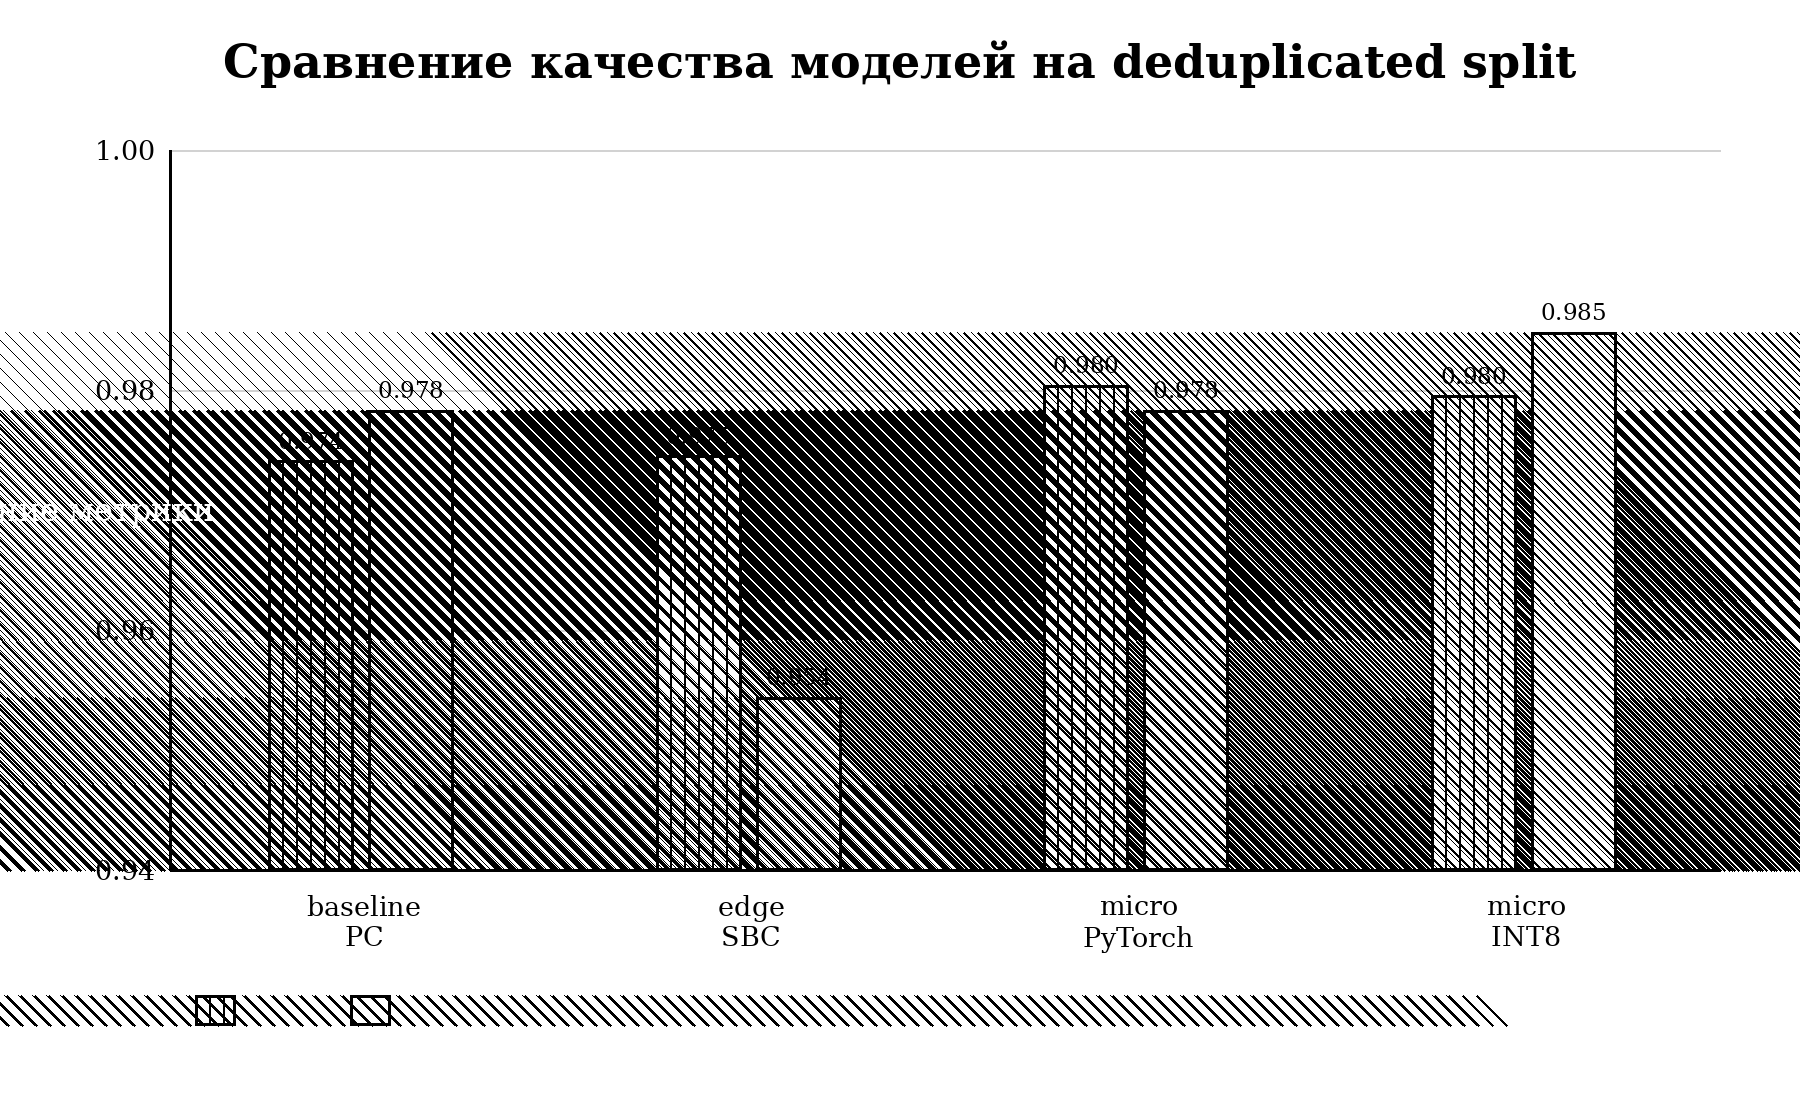
\includegraphics[width=0.92\textwidth]{figures/quality_comparison.png}
\caption{Сравнение качества моделей на deduplicated split}
\label{fig:quality}
\end{figure}

\begin{figure}[H]
\centering
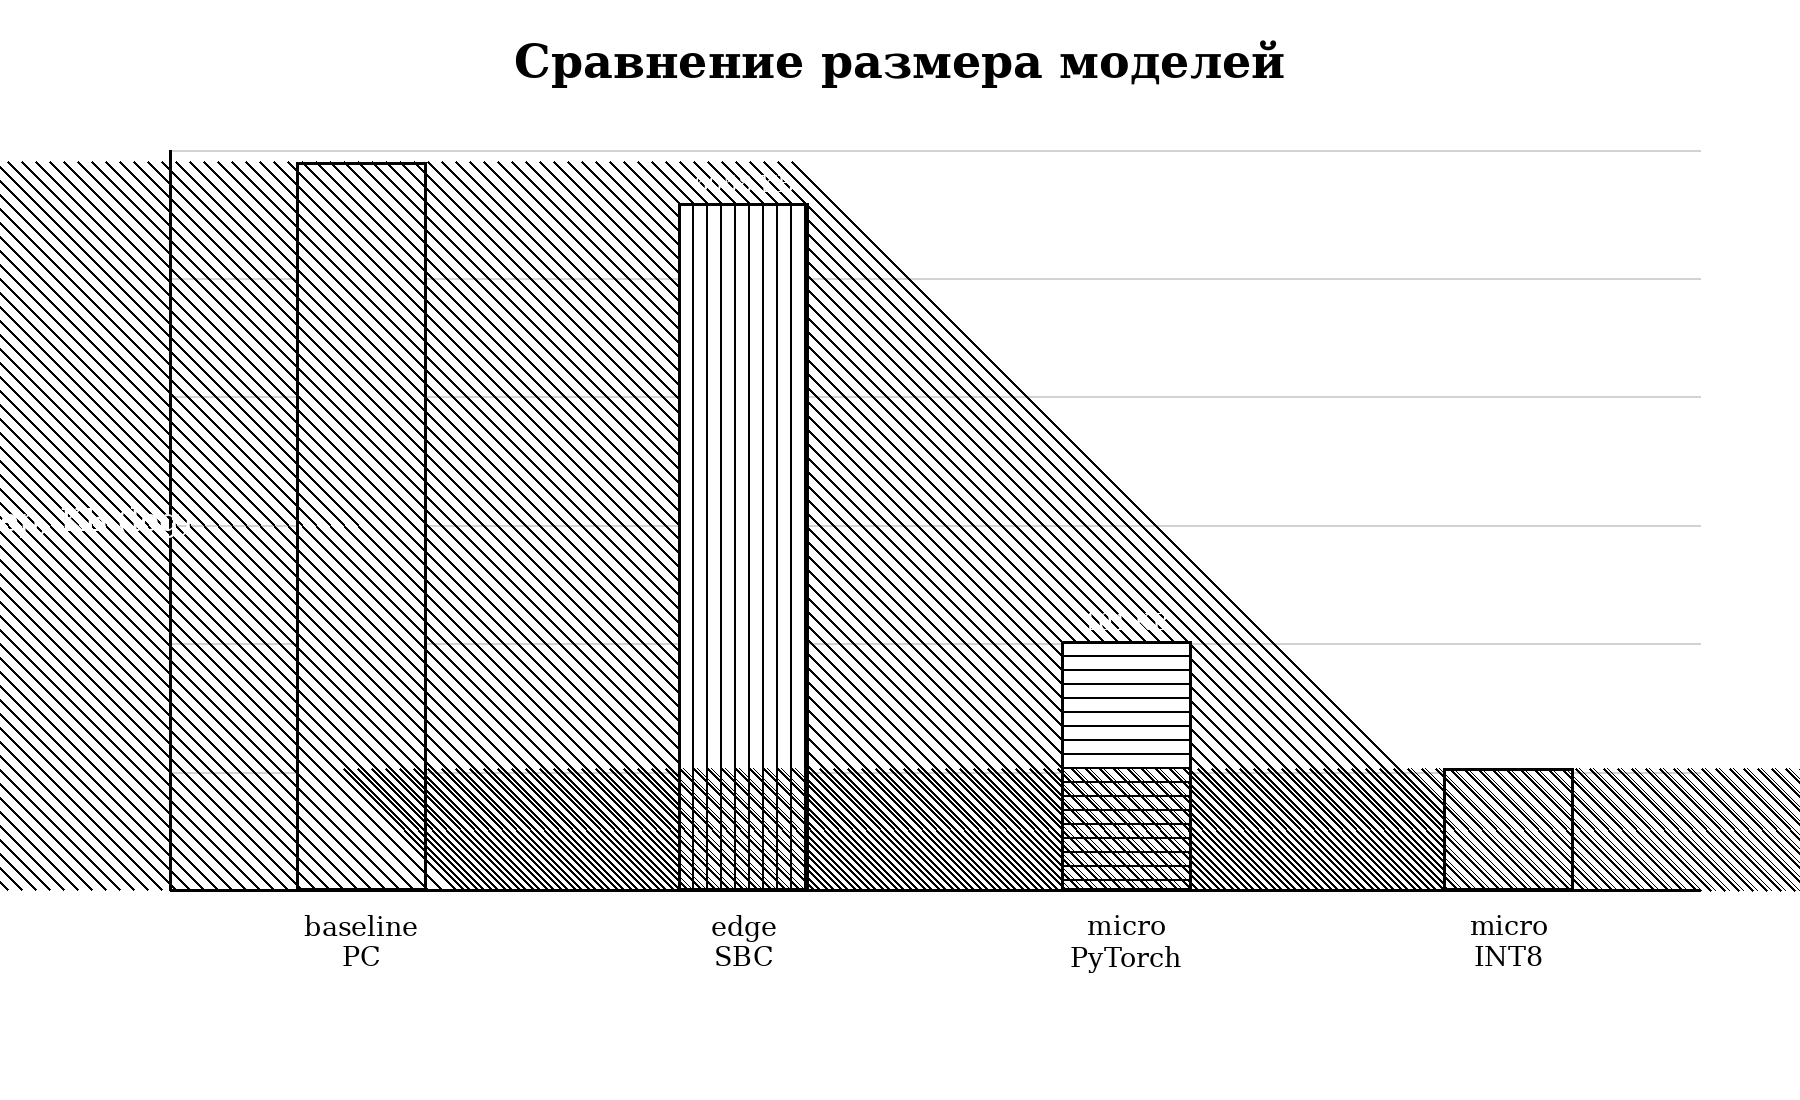
\includegraphics[width=0.92\textwidth]{figures/size_comparison_log.png}
\caption{Сравнение размеров моделей в KB, логарифмическая шкала}
\label{fig:size}
\end{figure}

Рисунки~\ref{fig:quality} и~\ref{fig:size} показывают, что micro-edge и INT8-вариант сохраняют близкое качество при резком уменьшении размера модели. Это является основным ресурсным выигрышем предложенной методики.

\subsection{Exact TFLite/INT8-конвертация}

Для micro-edge модели были получены два TFLite-файла:

\begin{itemize}
    \item \texttt{micro\_edge\_dedup\_exact\_fp32.tflite}: 97.0 KB;
    \item \texttt{micro\_edge\_dedup\_exact\_int8.tflite}: 31.0 KB.
\end{itemize}

TFLite INT8-модель использует входной тензор формы [1, 128, 128, 3] типа int8 и выходной тензор [1, 2] типа int8. В списке операций зафиксированы CONV\_2D, MAX\_POOL\_2D, MEAN, FULLY\_CONNECTED и DELEGATE. Набор операций выглядит простым для дальнейшей проверки в TFLite Micro/OpenMV-like режиме, однако фактическая совместимость требует проверки на целевом firmware.

Важно подчеркнуть, что модель не запускалась на OpenMV или Raspberry Pi. Полученный TFLite INT8-файл является корректным артефактом для следующего этапа проверки, но не является доказательством аппаратного внедрения.

\begin{figure}[H]
\centering
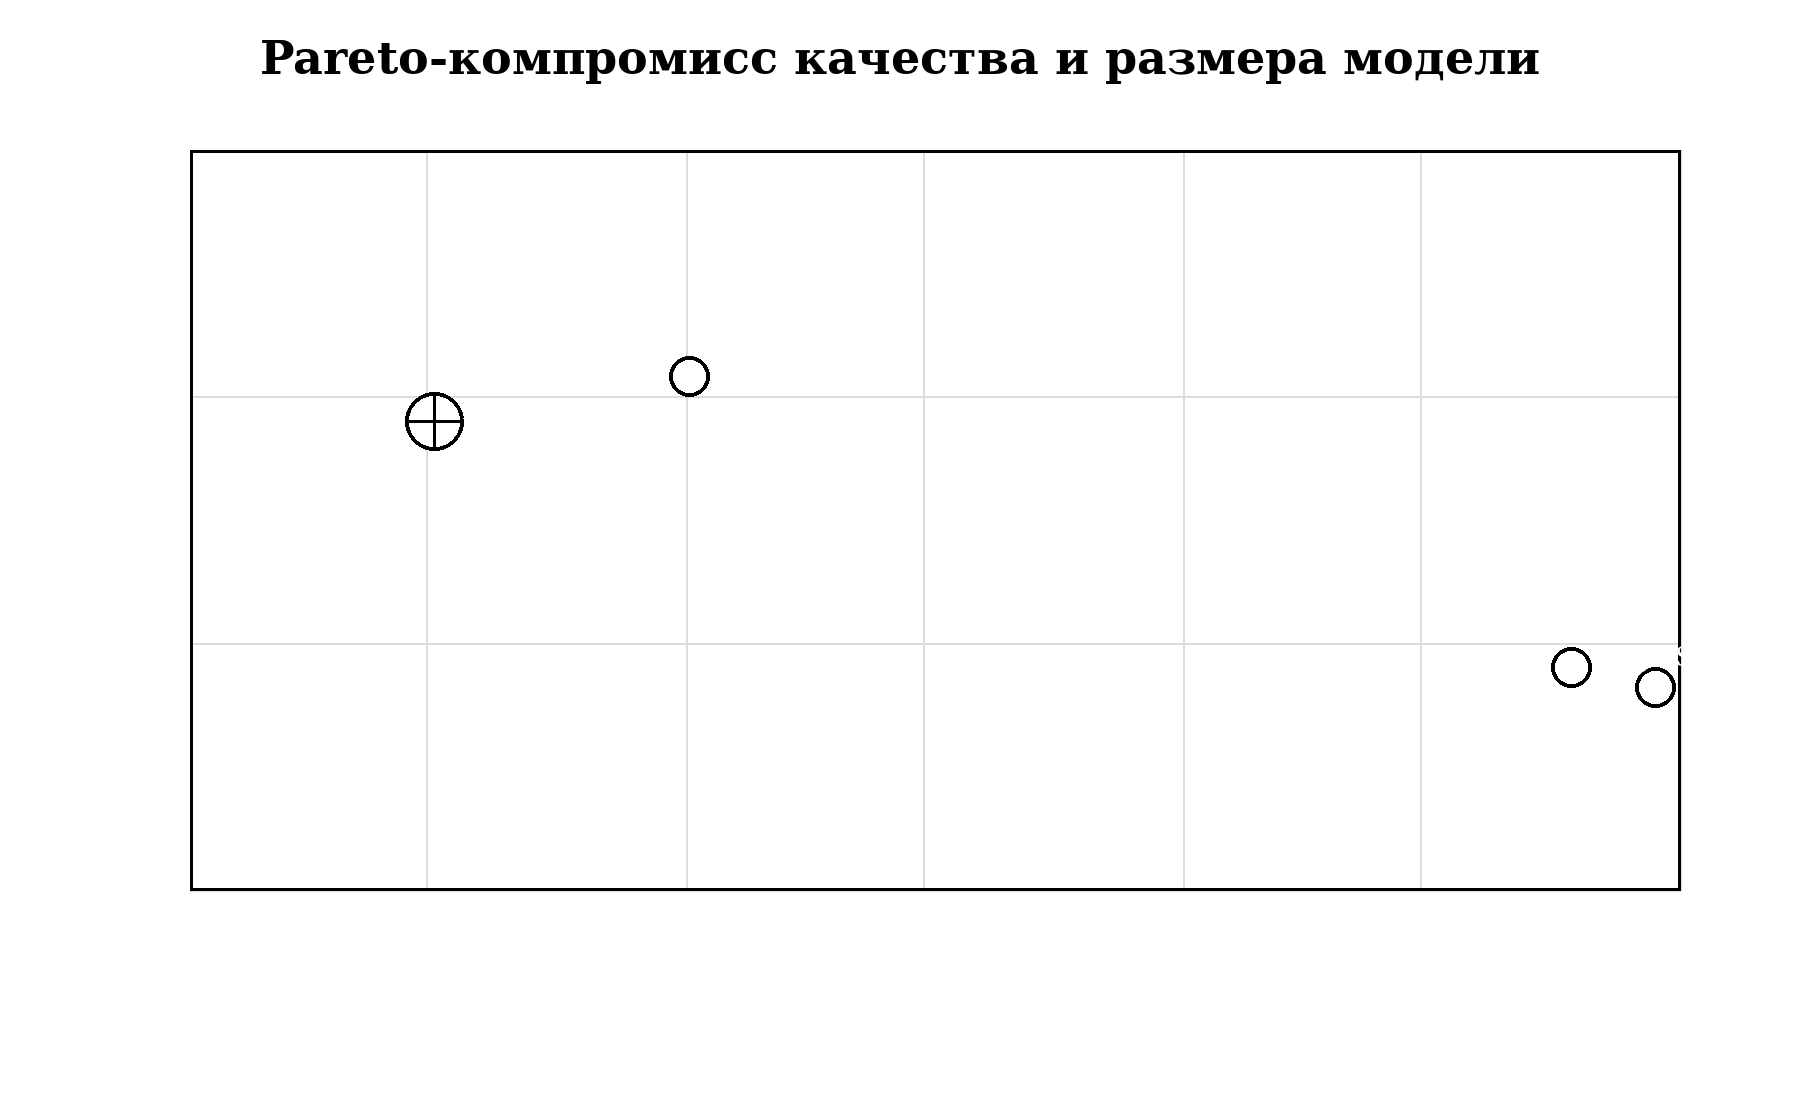
\includegraphics[width=0.86\textwidth]{figures/pareto_f1_size.png}
\caption{Pareto-анализ: F1 и размер модели}
\label{fig:pareto}
\end{figure}

\begin{figure}[H]
\centering
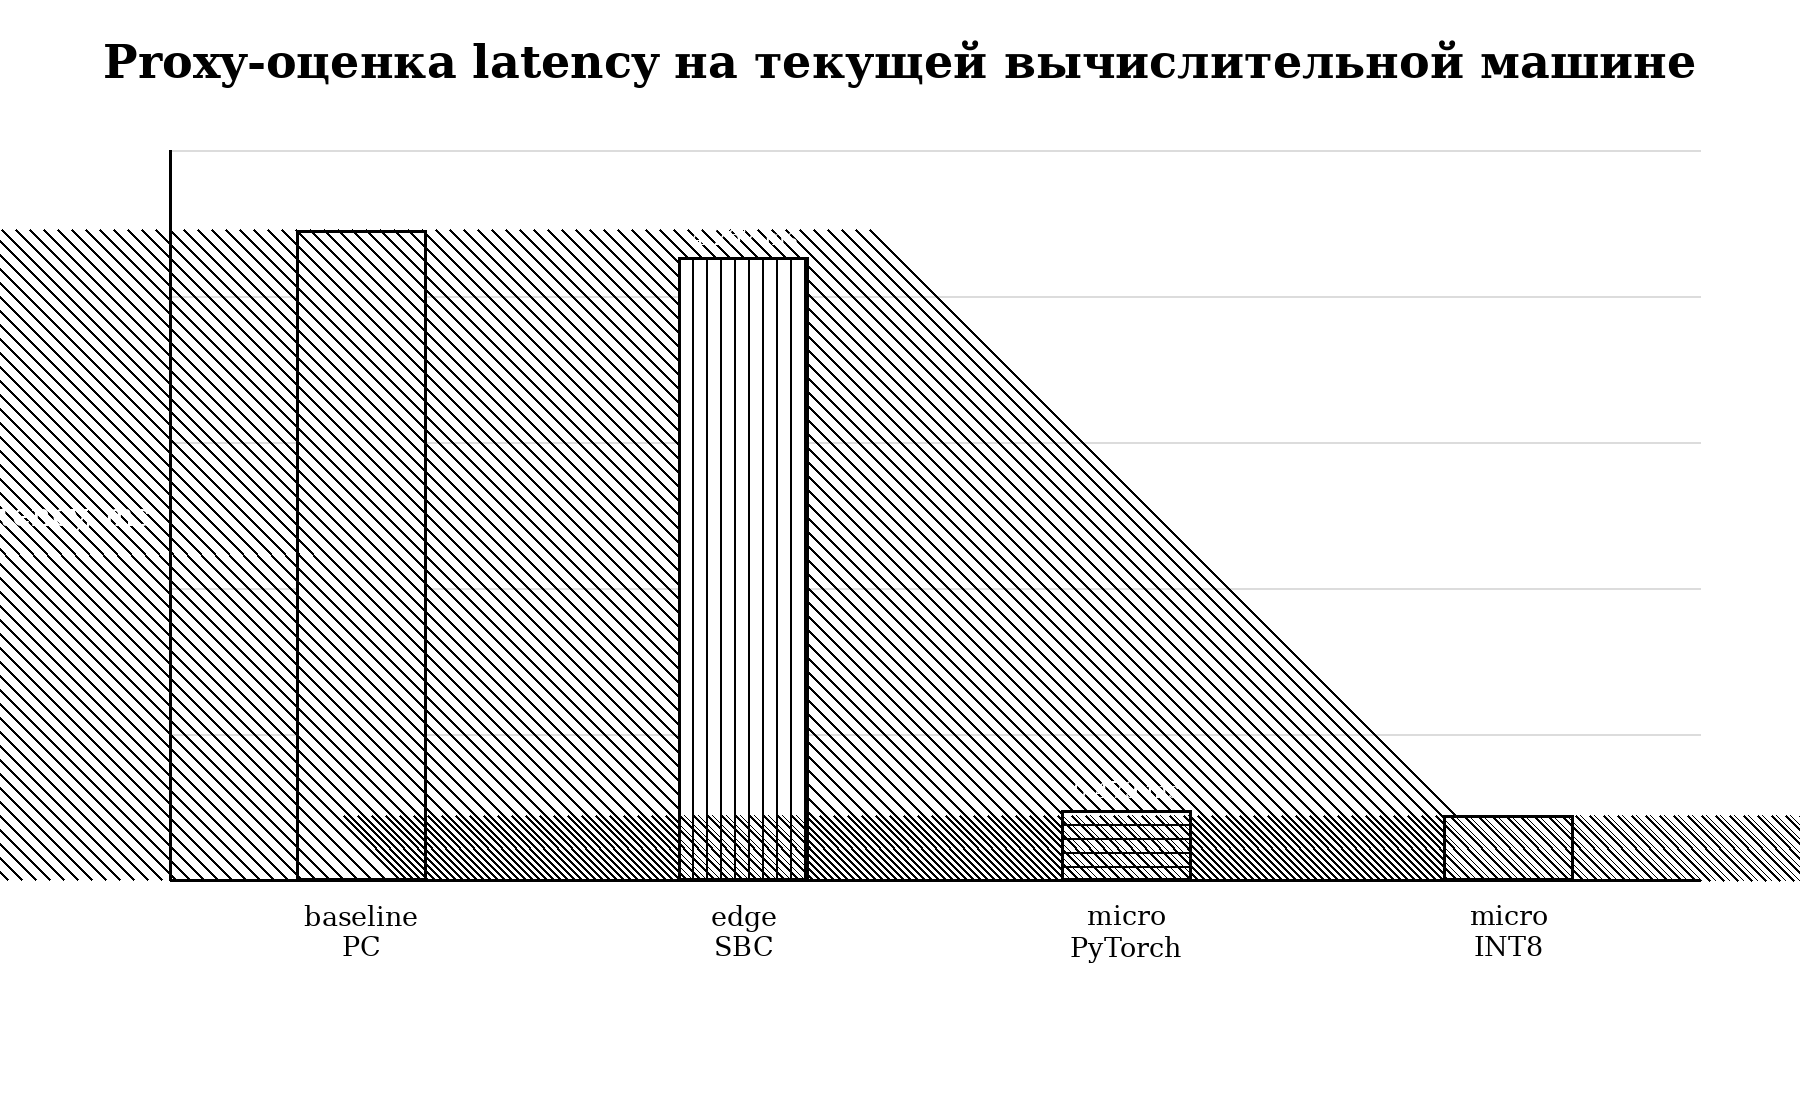
\includegraphics[width=0.86\textwidth]{figures/latency_comparison.png}
\caption{Сравнение latency, proxy-измерение}
\label{fig:latency}
\end{figure}

Pareto-анализ показывает, что INT8 micro-edge модель не является «лучшей вообще» по всем возможным критериям, но является наиболее ресурсно-эффективной в данном эксперименте: качество остается близким к PyTorch-модели, а размер и latency минимальны среди рассмотренных вариантов.

\subsection{Confidence-based triage}

Для промышленного контроля полезно не только классифицировать каждое изображение, но и отправлять сомнительные случаи на REVIEW. В confidence-based triage автоматическое решение принимается только при confidence выше заданного threshold. При меньшей уверенности изделие направляется на ручную проверку.

Для TFLite INT8-модели нулевой unsafe-error threshold найден не был. Лучший low-risk режим имел threshold 0.95, review rate 0.1723, accepted accuracy 0.9984 и 1 unsafe error. Это означает, что примерно 82.8\% изображений принимаются автоматически, а 17.2\% направляются на REVIEW. Такой режим может быть полезен, когда требуется снизить риск пропуска дефектов при сохранении высокой доли автоматической обработки.

\begin{table}[H]
\centering
\caption{Low-risk confidence triage для TFLite INT8}
\label{tab:triage}
\begin{tabular}{rrrrrr}
\toprule
Threshold & Coverage & Review rate & Accepted acc. & Accepted def. recall & Unsafe errors \\
\midrule
0.95 & 0.8277 & 0.1723 & 0.9984 & 0.9977 & 1 \\
\bottomrule
\end{tabular}
\end{table}

\begin{figure}[H]
\centering
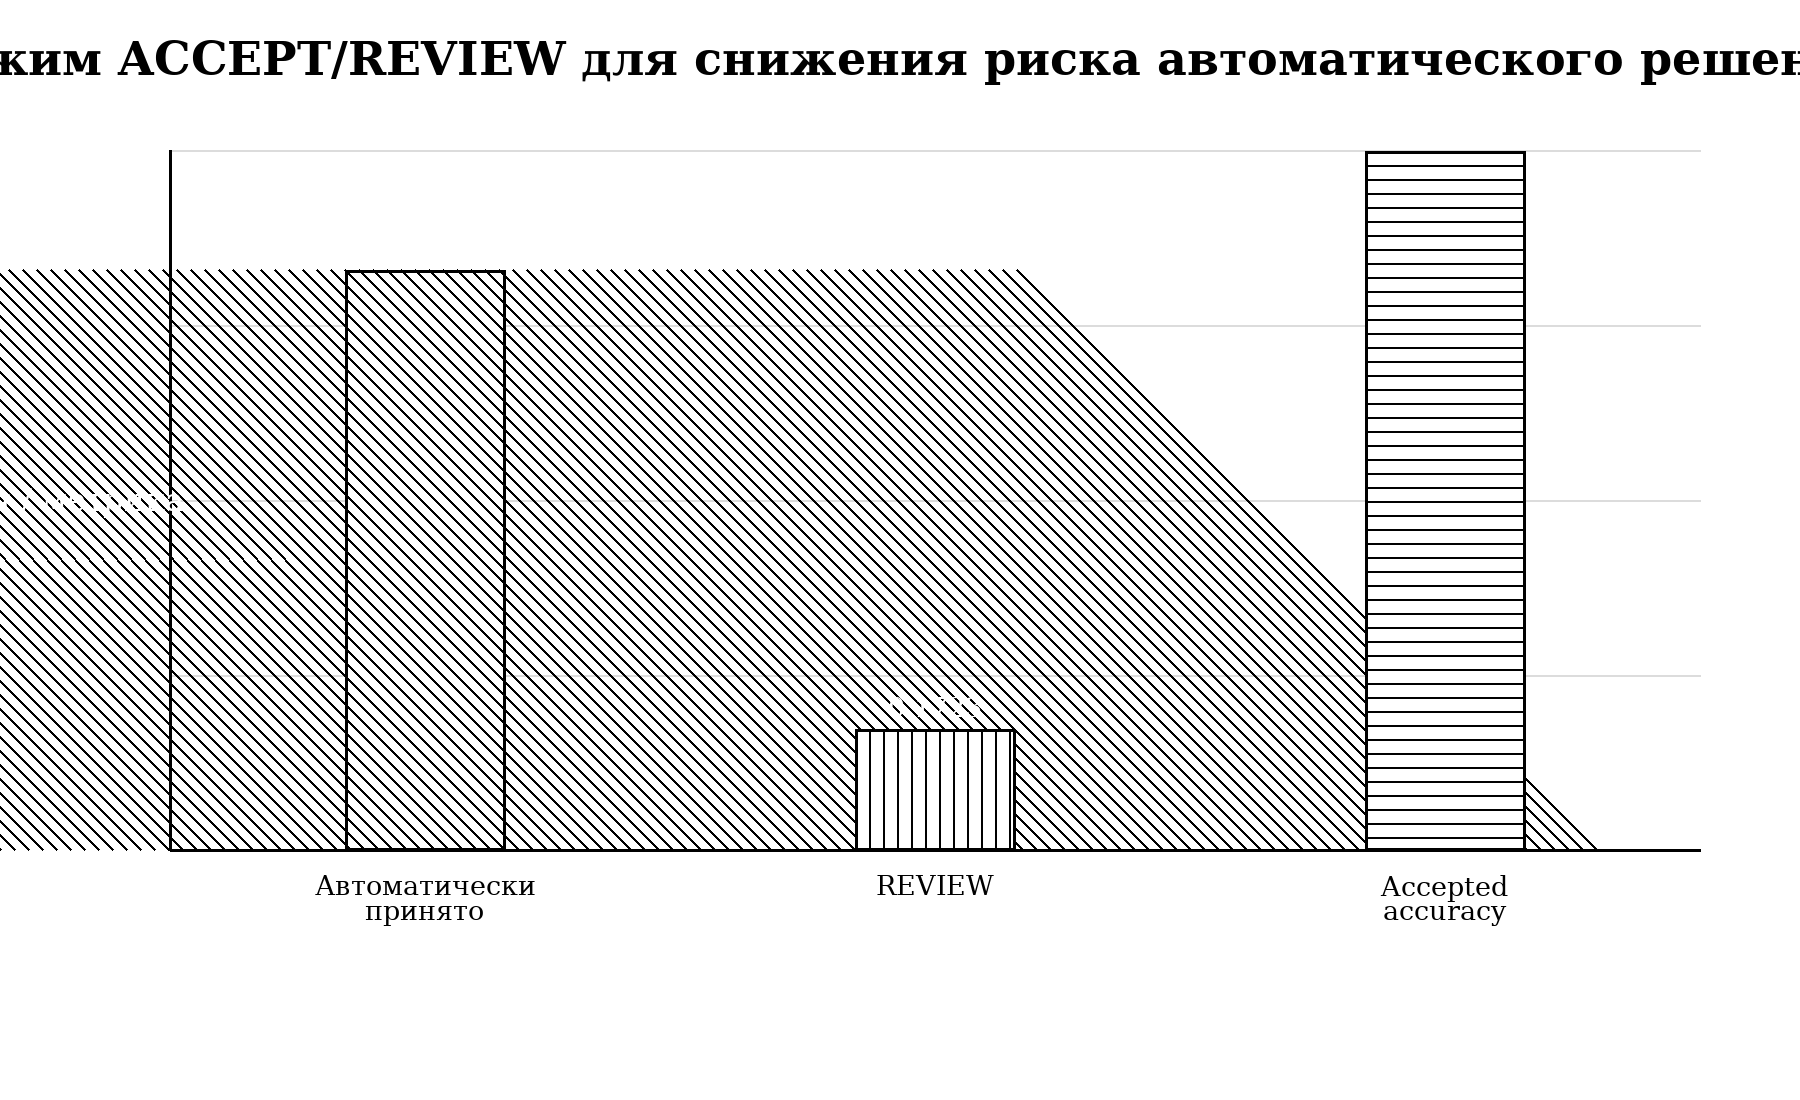
\includegraphics[width=0.86\textwidth]{figures/triage_tradeoff.png}
\caption{Компромисс confidence-based triage для INT8 micro-edge модели}
\label{fig:triage}
\end{figure}

\subsection{Сравнение с исходным split и опубликованными ориентирами}

После перехода от исходного split к deduplicated split метрики снизились. Для baseline accuracy уменьшилась на 0.0241, F1 на 0.0204. Для edge\_sbc accuracy уменьшилась на 0.0200, F1 на 0.0178. Для micro\_edge accuracy уменьшилась на 0.0163, F1 на 0.0141.

\begin{table}[H]
\centering
\caption{Изменение качества после перехода к deduplicated split}
\label{tab:delta}
\begin{tabular}{lrr}
\toprule
Профиль & $\Delta$ accuracy & $\Delta$ F1 \\
\midrule
baseline & -0.0241 & -0.0204 \\
edge\_sbc & -0.0200 & -0.0178 \\
micro\_edge & -0.0163 & -0.0141 \\
\bottomrule
\end{tabular}
\end{table}

Это снижение подтверждает, что исходный split мог завышать качество. Однако падение не является критическим: все модели сохраняют F1 выше 0.97. Поэтому deduplicated split дает более честную оценку, не отменяя применимости предложенной методики.

Опубликованные работы по этому датасету иногда сообщают accuracy выше 99\%, однако такие значения получены при иных условиях split, preprocessing и обучения. Поэтому в данной НИР они рассматриваются как ориентиры. Наиболее важным результатом настоящей работы является не абсолютное превосходство над SOTA, а демонстрация ресурсно-ориентированной адаптации с проверкой данных, TFLite/INT8 и triage.

\subsection{Практическая значимость и ограничения}

Практическая значимость работы состоит в подготовке воспроизводимого пайплайна для оценки моделей визуального контроля качества в условиях ресурсных ограничений. Такой подход может применяться при проектировании систем поддержки промышленного контроля, в том числе в решениях уровня Ретинар, где требуется учитывать не только качество модели, но и ограничения устройства и риск неуверенных решений.

Ограничения исследования следующие. Во-первых, latency является proxy на текущей машине, а не аппаратным замером на Raspberry Pi или OpenMV. Во-вторых, модели не запускались на реальных целевых устройствах. В-третьих, совместимость TFLite Micro/OpenMV firmware требует отдельной проверки. В-четвертых, average hash для near-duplicates является эвристикой. В-пятых, сравнение с опубликованными работами условное из-за различий split, preprocessing и epochs. В-шестых, датасет содержит однотипные изображения, поэтому перенос на другое производство требует валидации или дообучения.

\section*{Заключение}
\addcontentsline{toc}{section}{Заключение}

В работе разработана и экспериментально проверена методика адаптации моделей компьютерного зрения для контроля качества литых изделий на edge-устройствах разных ресурсных классов. Цель достигнута на уровне воспроизводимой исследовательской методики и экспериментальной проверки на deduplicated split.

Выполнен аудит исходного split и обнаружены cross-split duplicates и near-duplicates. Поэтому основным строгим результатом выбран deduplicated split, сформированный по группам похожих изображений. На нем micro-edge модель достигла accuracy 0.9767 и F1 0.9804 при размере 101.3 KB. Exact TFLite INT8-версия достигла accuracy 0.9754, F1 0.9795 и defective recall 0.9848 при размере 31.0 KB.

Полученные результаты подтверждают гипотезу: легковесная модель после адаптации и exact TFLite INT8-конвертации может сохранить приемлемое качество выявления дефектов при значительном снижении ресурсной стоимости. При этом работа не утверждает создание готовой промышленной системы. Для внедрения необходимы аппаратные измерения на целевых устройствах, проверка firmware-совместимости, multi-seed validation и тестирование на данных конкретной производственной линии.

\newpage
\addcontentsline{toc}{section}{Список использованных источников}
\bibliographystyle{plain}
\bibliography{references}

\newpage
\section*{Приложения}
\addcontentsline{toc}{section}{Приложения}

\subsection*{Приложение А. Схема воспроизводимого пайплайна}
\addcontentsline{toc}{subsection}{Приложение А. Схема воспроизводимого пайплайна}

Пайплайн исследования включает следующие этапы: загрузка фиксированного датасета; валидация структуры классов; аудит дубликатов; формирование deduplicated split; обучение трех профилей моделей; оценка качества; benchmark latency и размера; exact TFLite/INT8-конвертация; confidence-based triage; сравнение original split и deduplicated split; формирование итоговых таблиц.

\subsection*{Приложение Б. Основные артефакты эксперимента}
\addcontentsline{toc}{subsection}{Приложение Б. Основные артефакты эксперимента}

\begin{longtable}{p{0.36\textwidth}p{0.52\textwidth}}
\toprule
Артефакт & Расположение внутри проекта \\
\midrule
Clean split & каталог \texttt{processed\_clean} в dedup-training эксперименте \\
Веса baseline & файл \texttt{best.pt} для профиля \texttt{baseline\_pc\_dedup} \\
Веса edge\_sbc & файл \texttt{best.pt} для профиля \texttt{edge\_sbc\_dedup} \\
Веса micro\_edge & файл \texttt{best.pt} для профиля \texttt{micro\_edge\_dedup} \\
TFLite FP32 & FP32-экспорт micro-edge модели \\
TFLite INT8 & INT8-экспорт micro-edge модели \\
\bottomrule
\end{longtable}

Код, конфигурации, таблицы результатов, exact TFLite INT8-модель и инструкции
воспроизведения выделены в отдельный reference snapshot. Датасет Kaggle не
включается в репозиторий и скачивается отдельно. Ссылка на репозиторий:
[ДОБАВИТЬ ССЫЛКУ ПОСЛЕ ЗАГРУЗКИ]. Основные артефакты: clean split manifest,
metrics, tables, exact TFLite FP32/INT8, LaTeX/PDF НИР.

\subsection*{Приложение В. Примеры изображений датасета}
\addcontentsline{toc}{subsection}{Приложение В. Примеры изображений датасета}

\begin{figure}[H]
\centering
\begin{minipage}{0.42\textwidth}
\centering
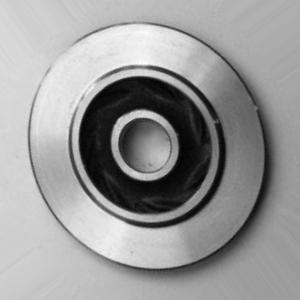
\includegraphics[width=0.86\linewidth]{figures/example_ok.jpeg}
\caption*{Класс \texttt{ok}}
\end{minipage}
\hfill
\begin{minipage}{0.42\textwidth}
\centering
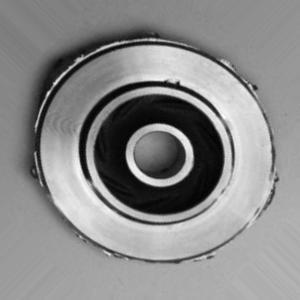
\includegraphics[width=0.86\linewidth]{figures/example_defective.jpeg}
\caption*{Класс \texttt{defective}}
\end{minipage}
\caption{Примеры изображений из clean test split}
\label{fig:examples}
\end{figure}

\subsection*{Приложение Г. Диагностические графики}
\addcontentsline{toc}{subsection}{Приложение Г. Диагностические графики}

\begin{figure}[H]
\centering
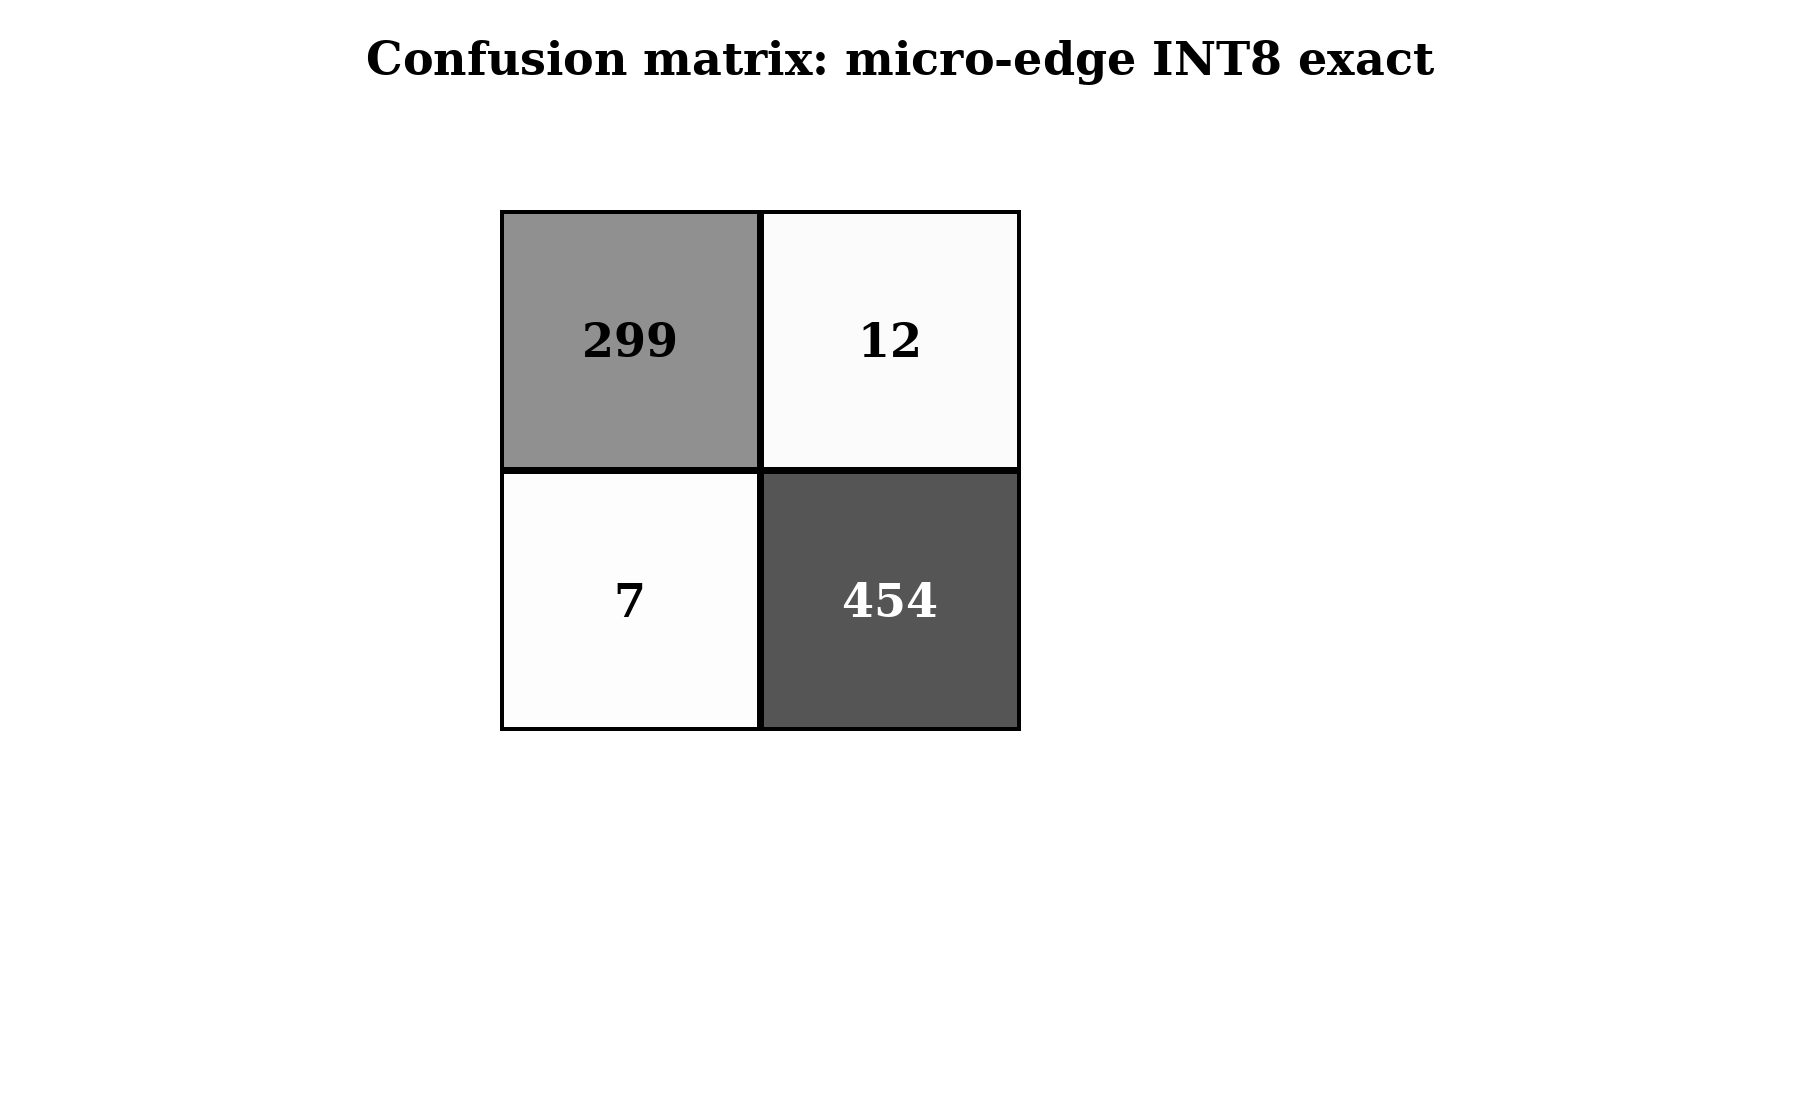
\includegraphics[width=0.72\textwidth]{figures/confusion_matrix_micro_int8.png}
\caption{Confusion matrix для exact TFLite INT8 модели на clean test}
\label{fig:cm}
\end{figure}

\subsection*{Приложение Д. Ограничения интерпретации}
\addcontentsline{toc}{subsection}{Приложение Д. Ограничения интерпретации}

Исходный split датасета содержит дубликаты и near-duplicates, поэтому результаты на нем следует использовать только как дополнительное сравнение. Основными результатами являются значения на deduplicated split. Latency является proxy-измерением на текущей машине. Raspberry Pi и OpenMV аппаратно не тестировались. TFLite INT8-файл требует дальнейшей проверки на целевом firmware. Обобщение на другие производства требует отдельной валидации.

\end{document}
